\documentclass[12pt,a4paper,twoside]{report}
\usepackage[left=3cm,right=3cm,top=2cm,bottom=3cm]{geometry}
\usepackage{pagenote}
\usepackage{algorithm}
\usepackage{algorithmic}
\usepackage{graphicx}
\usepackage[utf8]{inputenc}	% Para caracteres en español
\usepackage{amsmath,amsthm,amsfonts,amssymb,amscd}
\usepackage{multirow,booktabs}
\usepackage[table]{xcolor}
\usepackage{fullpage}
\usepackage{lastpage}
\usepackage{enumitem}
\usepackage{fancyhdr}
\usepackage{mathrsfs}
\usepackage{wrapfig}
\usepackage{setspace}
\usepackage{calc}
\usepackage{color,soul}
\usepackage{multicol}
\usepackage{cancel}
\usepackage[retainorgcmds]{IEEEtrantools}
\usepackage{xcolor}
\colorlet{shadecolor}{orange!15}
\parindent 0in
\parskip 12pt
\geometry{margin=1in, headsep=0.25in}
\theoremstyle{definition}
\newtheorem{defn}{Definition}
\newtheorem{reg}{Rule}
\newtheorem{exer}{Exercise}
\newtheorem{note}{Note}
\usepackage{listings}
\usepackage{spverbatim}
\usepackage{fancyvrb}
\usepackage{hyperref}
\usepackage{float} 
\usepackage{natbib}
\usepackage{tikz}
\usepackage{pgfplots}
\usepackage{pgfplotstable}
\usepackage{soulutf8}
\usepackage{color,soul}
\usepackage{xcolor}
\usepackage{tabularx}
\newtheorem{lemma}{Lemma}[section]
\newtheorem{theorem}{Theorem}[section]
\newtheorem{proposition}{Proposition}[section]
\newtheorem{definition}{Definition}[section]
\DeclareMathOperator*{\argmax}{argmax}
\usepackage[draft]{todo}
\newcommand{\fyTodo}[1]{\Todo[FY:]{\textcolor{orange}{#1}}}
\newcommand{\fyTodostar}[1]{\Todo*[FY:]{\textcolor{orange}{#1}}}
\newcommand{\fyDone}[1]{\done[FY]\Todo[FY:]{\textcolor{orange}{#1}}}
\newcommand{\fyDonestar}[1]{\done[FY]\Todo[FY:]{\textcolor{orange}{#1}}}
\pgfkeys{
    /tr/rowfilter/.style 2 args={
        /pgfplots/x filter/.append code={
            \edef\arga{\thisrow{#1}}
            \edef\argb{#2}
            \ifx\arga\argb
            \else
                \def\pgfmathresult{}
            \fi
        }
    }
}
\usepackage{mathtools,xparse}
\DeclarePairedDelimiter{\abs}{\lvert}{\rvert}
\DeclarePairedDelimiter{\norm}{\lVert}{\rVert}
\NewDocumentCommand{\normL}{ s O{} m }{%
  \IfBooleanTF{#1}{\norm*{#3}}{\norm[#2]{#3}}_{L_1}%
}

\begin{document}
\begin{center}
{\LARGE \bf Combination of generic and specific}\\
\end{center}
\setlength{\belowdisplayskip}{8pt} \setlength{\belowdisplayshortskip}{8pt}
\setlength{\abovedisplayskip}{8pt} \setlength{\abovedisplayshortskip}{8pt}
\setlist{nosep}
\setlength{\parskip}{0.1cm}
\setlength{\parindent}{1em}
\section*{Word Level Adaptive Domain Adaptation}
Let $h$ the output of the pretrained encoder, the adapted representation for domain $k$ will be $h' = h + a_k(h)$, meaning that all words in all sentences for domain $k$ will use the adapter module $a_k$.  A ``gated'' version uses $h' = h + a_k(h) * z_k$\footnote{More precisely, $a_k(h) = \sum_{l} a_{kl}(h)$, where the summation runs over layers, see Figure \ref{fig:1}} \fyTodo{$a_k(h)=$ somme tous les composants résiduels} where $z_k$ is also a function of $h$ taking values in $[0,1]$. More precisely, $h$ and $h'$ are sequences of context vectors and the combination is performed element-wise, yielding:
\begin{equation}
  h'(w) = h(w) + a_k(h(w)) * z_k(h(w)). \label{eq:gated-residual}
\end{equation}

In Word Level Adaptive Domain Adaptation, $z_k(h(w))$ is designed to reflect the ``topicality'' of  word $w$ is in domain $k$: the more likely $w$ is in domain $k$, the larger $z_k(h(w))$ is. The word-level adaptive domain adaptation aims to reduce the variation caused by $a_k$ to the adapted context vector $h'$ (compared to $h$) for words that are not typical of domain $k$. For a domain, there are 2 type of non-topical words: out-of-domain words that rarely or never appear in the in-domain texts; or frequent words that appear equally frequently in many domains. \fyTodo{This is like a poor Tf-idf - can be because tf is small or because idf is small} 

\fyTodo{Experiment: compute posterior probability of words that have poor $tf-idf$ to verify the gating operation}. 

By reusing the learned generic representation for the non-topical words, we can at least bound the risk of poor predictions in case of out-of-domain words by the risk of the learned generic model (see below).
\begin{figure}[h!]
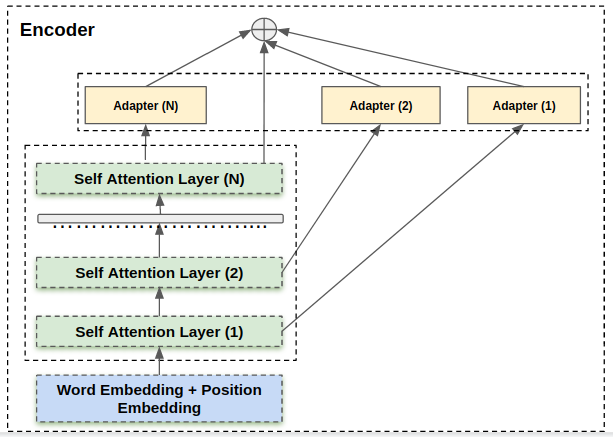
\includegraphics[scale=0.5]{highway_residual}
\caption{Highway residual layer}
\label{fig:1}
\end{figure}

\section*{Training process}
The training process comprises thre main steps:
\begin{itemize}
\item Pretraining a generic model with a mixed corpora.
\item Training a domain classifier on top of the encoder and decoder; during this step, the parameters of the generic model are frozen. This model computes the posterior domain probability $p(k|h(w))$ for each word $w$ based on the representation computed by the last layer.
We applied domain classifiers to the output of the encoder and to the output of the decoder, i.e, at the last self-attention layer of the encoder and the attention layer of the decoder.There are 2 classifiers which are placed in the top of the encoder and in the top of the decoder.
$$z^{enc}_k(w^{src}_t) = p(d=k| h_{enc}(w^{src}_t))$$
where $h_{enc}(w^{src}_t)=Enc(x)(w^{src}_t)$ and 
$$z^{dec}_k(w^{tgt}_t) = p(d=k| h_{dec}(w^{tgt}_t))$$  
where $h_{dec}(w^{tgt}_t)=Dec(x,y_{i<t})(w^{tgt}_t)$

\fyTodo{Which layer, which classifier ?}
\item Training parameters of adapters with in-domain data separately while freezing the parameters of the generic model and of the domain classifiers.
\end{itemize}
During the inference, $z_k$ is used to regulate the strength of the adapter module as suggested in equation~\ref{eq:gated-residual}.

\section*{Weakness of the method}

This method depends crucially to the quality of the classifier $p(k|h(w))$. Moreover, the classifier can fail to detect in-domain words in the case of polysemous words. For example, the word "joint" in ``joint stereo'', ``joint sprain'' and ``joint project'' correspond to multiple translations such as "joint" and "articulaire" in French. In the unbalanced dataset as the mixed corpora (6 in-domain corpora),  "joint stereo" is hardly to be detected as in IT domain, therefore "joint stereo" does not profit the finetuning's effect even being translated with the adapters of IT domain.

\section*{Analysis on the risk of new method}

The combination of a generic representation and a residual adapter is defined as follows:
\begin{equation}
  h' = h + a_k(h) \label{eq:residual-adapter}
\end{equation}

where $h$ is the output of shared ``generic'' layers, i.e $h=M(x,y)$, $M: \mathbb{X} \times \mathbb{Y} \rightarrow \mathbf{\Omega}\subset \mathbb{R}^{d_{model}}$, $a_k$ is the residual adapter defined as a function $a_k: \mathbb{R}^{d_{model}} \rightarrow \mathbb{R}^{d_{model}}$.

The poor performance of fine-tuned models with a residual layer happens as the value of $a_k(h)$ of an out-of-domain example $(x^{adv}, y^{adv})$ is adversarial to the model. Indeed, by fine-tuning the adapter with only in-domain data, $a_k$ never encounters adversarial examples, which makes it error-prone in the face of out-of-domain examples. The intuition of wada is that we control the weight of $a_k(h)$ in the combination, we can hope to reduce the wrong belief of $a_k$ on adversarial examples. To implement this idea, we  investigate a convex combination of the generic and the residual layers, and define the adapted representation to be:

\begin{equation}
h' = h + a_k(h) * f(z_k), 
\label{eq:2}
\end{equation}

\noindent{}where
\begin{itemize}
\item $z_k = p(d=k | h=M(x,y)) = p_k(h)$ with $p: \mathbf{\Omega} \rightarrow \mathbf{\Delta}^{K}$. In the sequence to sequence version, there are 2 classifiers which are placed in the top of the encoder and in the top of the decoder.
$z^{enc}_k(w_t) = p(d=k| h_{enc}(w_t)=Enc(x)(w_t))$ and $z^{dec}_k(w_t) = p(d=k| h_{dec}(w_t)=Dec(y_t,x,y_{i<t})(w_t))$
\fyTodo{Attention à $x$ et $y$}
\item f is an activation function $f: [0,1] \rightarrow [0,1]$ 
\end{itemize}

We assume that the hidden distribution of a multi-domain problem limited to an unknown mixture of $K$ in-domain distribution, i.e, $$P(x,y) = \sum_{k\in[1..K]}P(x,y|d=k)P(d=k)$$. We denote also $D_k$ the distribution of domain k $P(x,y|d=k)$

We define some important constants:
\begin{itemize}
\item Inseparability of domains over a fixed representation space $\Omega$
\begin{equation}
  \begin{split}
  \mathbb{\varepsilon}_{insep} = \min_{p} \sum_{k\in[1..K]} \mathbb{E}_{x,y \sim \sum_{i\in [1..K]} \mathcal{D}_{i}*p(d=i)}(\mathbf{1}_{d\neq k} p(k|h))
  \end{split}
  \end{equation}
\item Inseparability of domain k from other domains over a fixed representation space $\Omega$
  \begin{equation}
  \begin{split}
  \mathbb{\varepsilon}_{insep}^k = \min_{p} \mathbb{E}_{x,y \sim \sum_{i\in [1..K]} \mathcal{D}_{i}*p(d=i)}(\mathbf{1}_{d\neq k} p(k|h))
  \end{split}
  \end{equation}
\item Risk of the generic model: $\mathbb{R} = \mathbb{E}_{(x,y \sim \sum_{k}p(x,y|d=k)p(d=k)) \sim \mathcal{D}}(l(M(x,y_{<t}), y_t))$ \fyTodo{wrt to which distribution ?}
\item $\mathbf{\Omega_{k,p_{0}}} = \lbrace h | z_k = p_\theta(k|h) < p_0\rbrace$.
\item Risk of the adapted model for the in-domain test set:
  $$R_k = \mathbb{E}_{x,y \sim \mathcal{D}_k} [l(h + a_k(h) * f(z_k), y)]$$
\end{itemize}

We also have two assumptions on the regularity of the activation and the loss functions:
\begin{itemize}
\item $a_k$ is bounded in sense of $\normL{a_k(h)} < M$
\item the loss function is bounded in sense of $l(h,y) < A$ $\forall h \in \Omega + \mathbb{B}(M)$ where $\mathbb{B}(M)=\lbrace x\in \mathbb{R}^{d_{model}} | \normL{x}<M \rbrace$ and $A+_{\alpha}B = \lbrace x+ \alpha y  | \alpha \in [0..1], x \in A, y \in B \rbrace$  \fyTodo{why not $l(h,y) < A$ ?}
  $\forall x,y$
\end{itemize}

Finally, we assume that the classifier is good enough, i.e, $$err_k(p) = \mathbb{E}_{x,y \sim \sum_{i\in [1..K]} \mathcal{D}_{i}*p(d=i)}(\mathbf{1}_{d\neq k} p(k|h)) < \varepsilon_{insep}^k + \gamma$$ $\forall k$ with $\gamma$ sufficiently small.
We then evaluate the risk of the model adapted to domain $k$ with residuals $a_k$ for arbitrary examples from $K$ domains:
\begin{equation}
\begin{split}
  R(M,a_k) &= \mathbb{E}_{x,y}[l(h + a_k(h) * f(z_k),y)] \\
  &= \mathbb{E}_{x,y}[l(h + a_k(h) * f(z_k),y)\mathbf{1}_{\mathbf{\Omega_{k,p_{0}}}}(h)] + \\
  &+ \mathbb{E}_{x,y}[l(h + a_k(h) * f(z_k),y) \mathbf{1}_{\mathbf{\Omega_{k,p_{0}}^{c}}}(h)]
\end{split}
\end{equation}

By designing a suitable activation function, we can map $f: [0,p_{0}] \rightarrow [0,\delta]$. Then with $\delta$ is small enough we can have an approximation of the first term:
\begin{equation}
\mathbb{E}_{x,y}[l(h + a_k(h) * f(z_k),y)\mathbf{1}_{\mathbf{\Omega_{k,p_{0}}}}(h)] \approx{} \mathbb{E}_{x,y}[l(h,y)\mathbf{1}_\mathbf{\Omega_{k,p_{0}}}(h)] \leq \mathbb{E}_{x,y}[l(h,y)] = R
\label{eq:4}
\end{equation}
The second term: $ L = \mathbb{E}_{x,y}[l(h + a_k(h) * f(z_k),y) \mathbf{1}_{\mathbf{\Omega_{k,p_{0}}^{c}}}(h)]$ can be bounded as follows:
\begin{equation*}
\begin{split}
L &= \displaystyle{\mathop{\sum}_{k'}\mathbb{E}_{x,y \sim p(.|d=k')}[l(h } + a_k(h) * f(z_k),y) * \mathbf{1}_{\mathbf{\Omega_{k,p_{0}}^{c}}}(h)]p(d=k') \\
	& \leq \displaystyle{\mathop{\sum}_{k' \neq k}} A * \mathbb{E}_{x,y \sim p(.|d=k')} [\mathbf{1}_{\mathbf{\Omega_{k,p_{0}}^{c}}}(h)]P(d=k') \\
	& \quad + \mathbb{E}_{x,y \sim p(.|d=k)}[l(h + a_k(h) * f(z_k),y) * \mathbf{1}_{\mathbf{\Omega_{k,p_{0}}^{c}}}(h)]P(d=k) \\
	&\leq A * \frac{\mathbb{\varepsilon}_{insep}^k + \gamma}{p_{0}} + R_k * P(d=k)
\end{split}
\label{eq:5}
\end{equation*}

The last inequality is verified since:
\begin{equation}
\begin{split}
\displaystyle{\mathop{\sum}_{k' \neq k}} A * \mathbb{E}_{x,y \sim p(.|d=k')} [\mathbf{1}_{\mathbf{\Omega_{k,p_{0}}^{c}}} (h)]P(d=k') &\leq A * \displaystyle{\mathop{\sum}_{k' \neq k}} \mathbb{E}_{x,y \sim p(.|d=k') } [\frac{p_k(h)}{p_0}]P(d=k') \\
		& = \frac{A}{p_0} \mathbb{E}[\mathbf{1}_{d\neq k}p_k(h)] \\
		& \leq \frac{A}{p_0} (\mathbb{\varepsilon}_{insep}^k + \gamma)
\end{split}
\end{equation}
because
$$ \mathbf{1}_{\mathbf{\Omega_{k,p_{0}}^{c}}}(h) \leq \frac{p_k(h)}{p_0} $$
Combining the inequality \ref{eq:4} and the inequality \ref{eq:5} we obtain the risk in general case of the adapted model $(M,a_k)$ $$R(M,a_k) \leq R + A * \frac{\mathbb{\varepsilon}_{insep}^k + \gamma}{p_0} + P(d=k)R_k$$

If we the original version of the residual adapter, with the same assumption in the regularization of the adapter, the bound of the risk of translating out-of-domain is only A (the bound of loss function). By using adaptive version, we reduce A by factor $\frac{p_0}{\epsilon^k_{insep}+\gamma}$ which is high if we choose $p_0$ is high enough, the domains are distant and the classifier is good enough. 

Furthermore $ \varepsilon^k_{insep} < \varepsilon_{insep} $ which is the minimum of the error expectation over the hypothesis space of the classifier. With a trivial prediction $[\frac{1}{K},..,\frac{1}{K}]$ we have an error expectation equal to 0.5. Therefore, $\varepsilon_{insep} \leq 0.5$, i.e, $\varepsilon^k_{insep} < 0.5$. In the worst case where domains in the mixture are very close, we are still able to reduce the risk of predicting out-of-domain examples by a factor of 2.
\fyTodo{I sort of buy the equations but then so what ? We should may be compare with non-adaptive ?}

\end{document}


